\documentclass[12pt, a4paper]{article}

\usepackage{graphicx}


\title{Notulensi Pertemuan}
\author{BMKG 2}
\date{3 July 2022}

\begin{document}
\maketitle

\begin{tabbing}
\textbf{Hari/Tanggal}\quad\= Minggu, 3 July 2022 \\
\textbf{Waktu} \>19.30 - 21.00 \\
\textbf{Tempat}\> Zoom Meeting
\end{tabbing}

Agenda pertemuan hari ini adalah:
\begin{enumerate}
\item perkenalan diri masing masing,
\item pembahasan mekanisme demo day,
\item eksplorasi dan pembahasan dataset
\end{enumerate}

\bigskip 
Pada pertemuan ini kami membahas tentang isi dari dataset BMKG yang diberikan dan mencari referensi terkait parameter yang terdapat di dalam dataset tersebut, seperti yang diketahui bersama, kami mendapatkan dataset BMKG/Weather yang berasal dari OpenWeather. Data tersebut memuat informasi berbagai macam parameter hasil pengukuran lapangan setiap 10 menit sekali di wilayah Denpasar, Bali.


\medskip 
Setelah kami cermati bersama ternyata ada beberapa parameter pengukuran yang tidak mempunyai data yang lengkap ataupun cenderung kosong pada banyak kejadian. Oleh karena itu kami sepakat untuk tidak menggunakan beberapa parameter tersebut. Pada pertemuan kali ini kami juga menetapkan parameter awal yang akan kami gunakan sebagai input dan target dari model yang akan kami kembangkan. 

\medskip 
Karena keterbatasan waktu untuk melakukan eksplorasi dataset dan terasa terlalu awal untuk menentukan parameter sebagai input dan target, kami sepakat untuk mengadakan pertemuan selanjutnya pada tanggal \textbf{9 Juli 2022} dengan tujuan agar setiap individu anggota kelompok dapat mempelajari dataset lebih baik sehingga pada pertemuan selanjutnya penentuan parameter input dan target dapat menjadi lebih matang.

\pagebreak
Agenda pertemuan selanjutnya adalah:
\begin{enumerate}
\item eksplorasi dataset lebih lanjut (Pemahamannya)
\item pembagian tugas per individu (Koding, Dokumentasi, Presentasi, Proposal)
\end{enumerate}

\bigskip
\section*{Dokumentasi}

\begin{figure}[h!]
  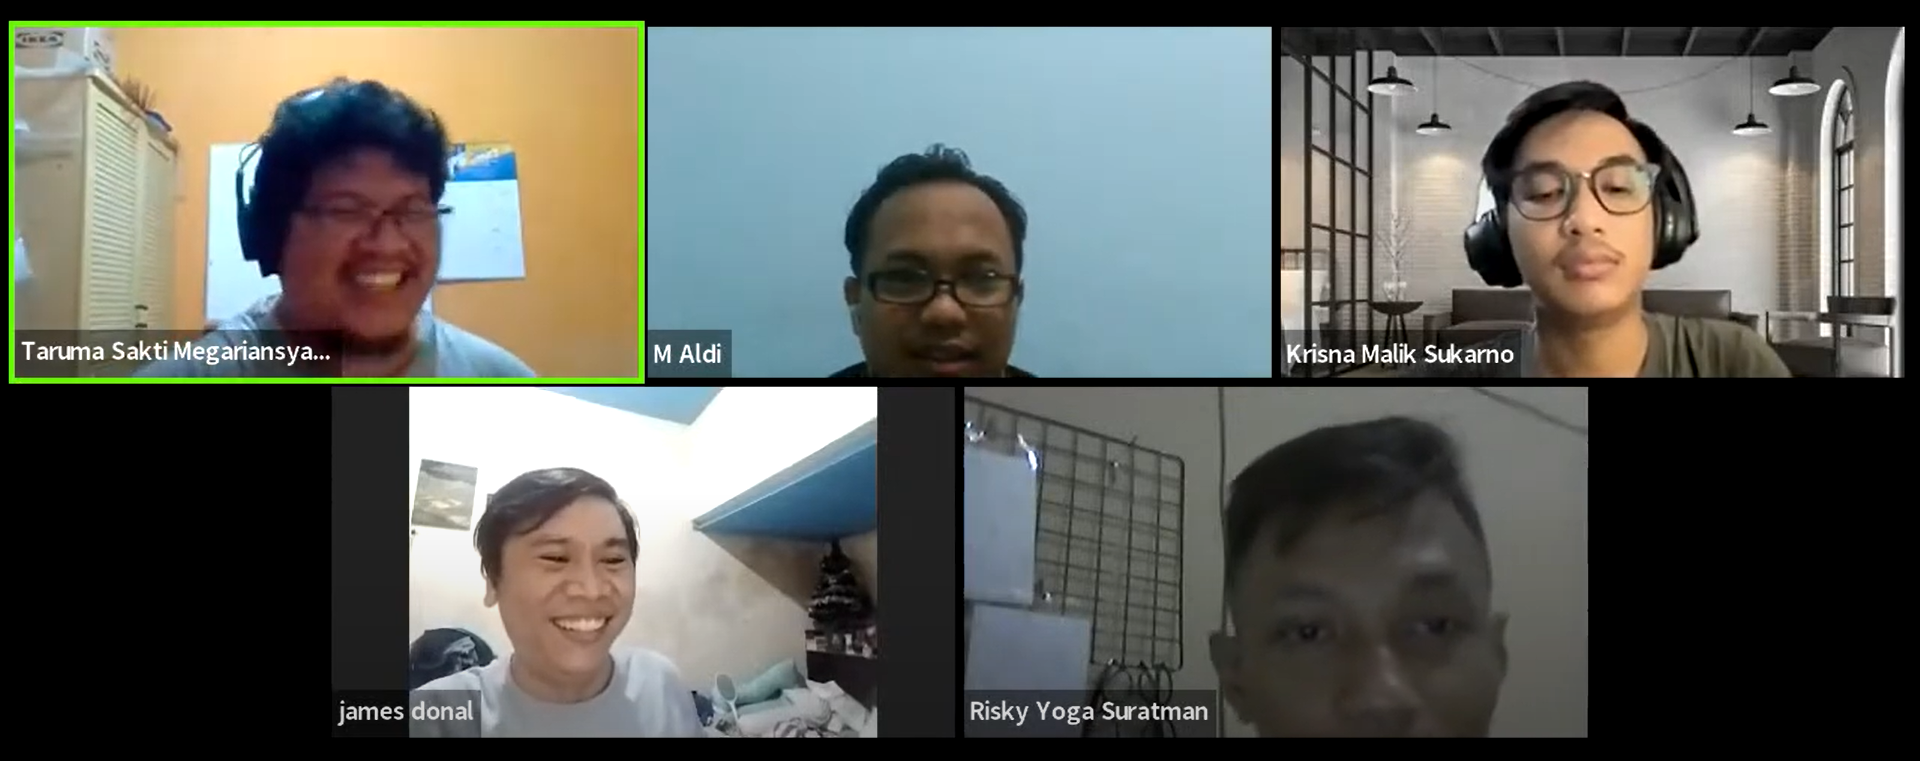
\includegraphics[width=\linewidth]{pert-1.png}
  \caption{Diskusi Kelompok}
\end{figure}

\begin{figure}[h!]
  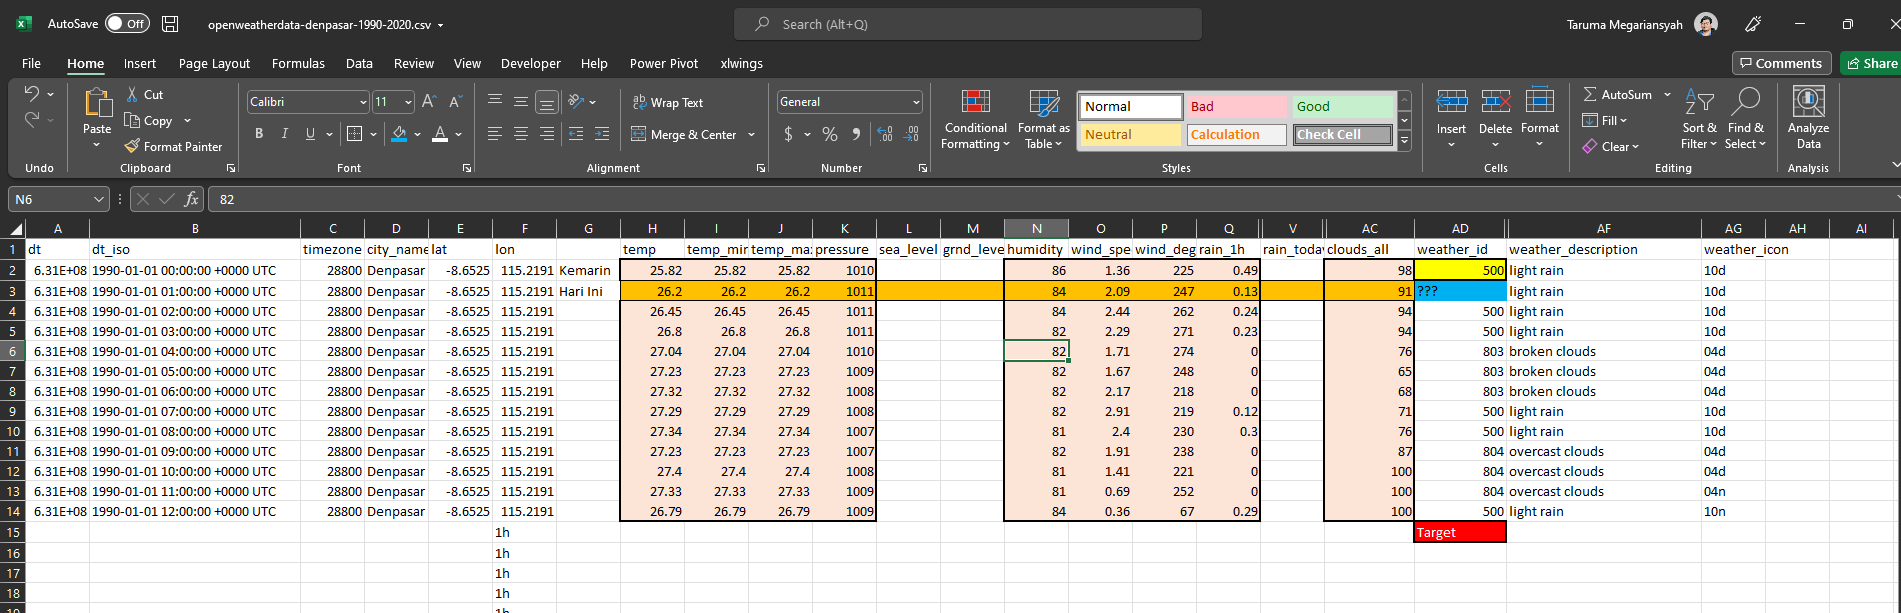
\includegraphics[width=\linewidth]{pert-11.png}
  \caption{Eksplorasi Dataset}
\end{figure}

\begin{figure}[h!]
  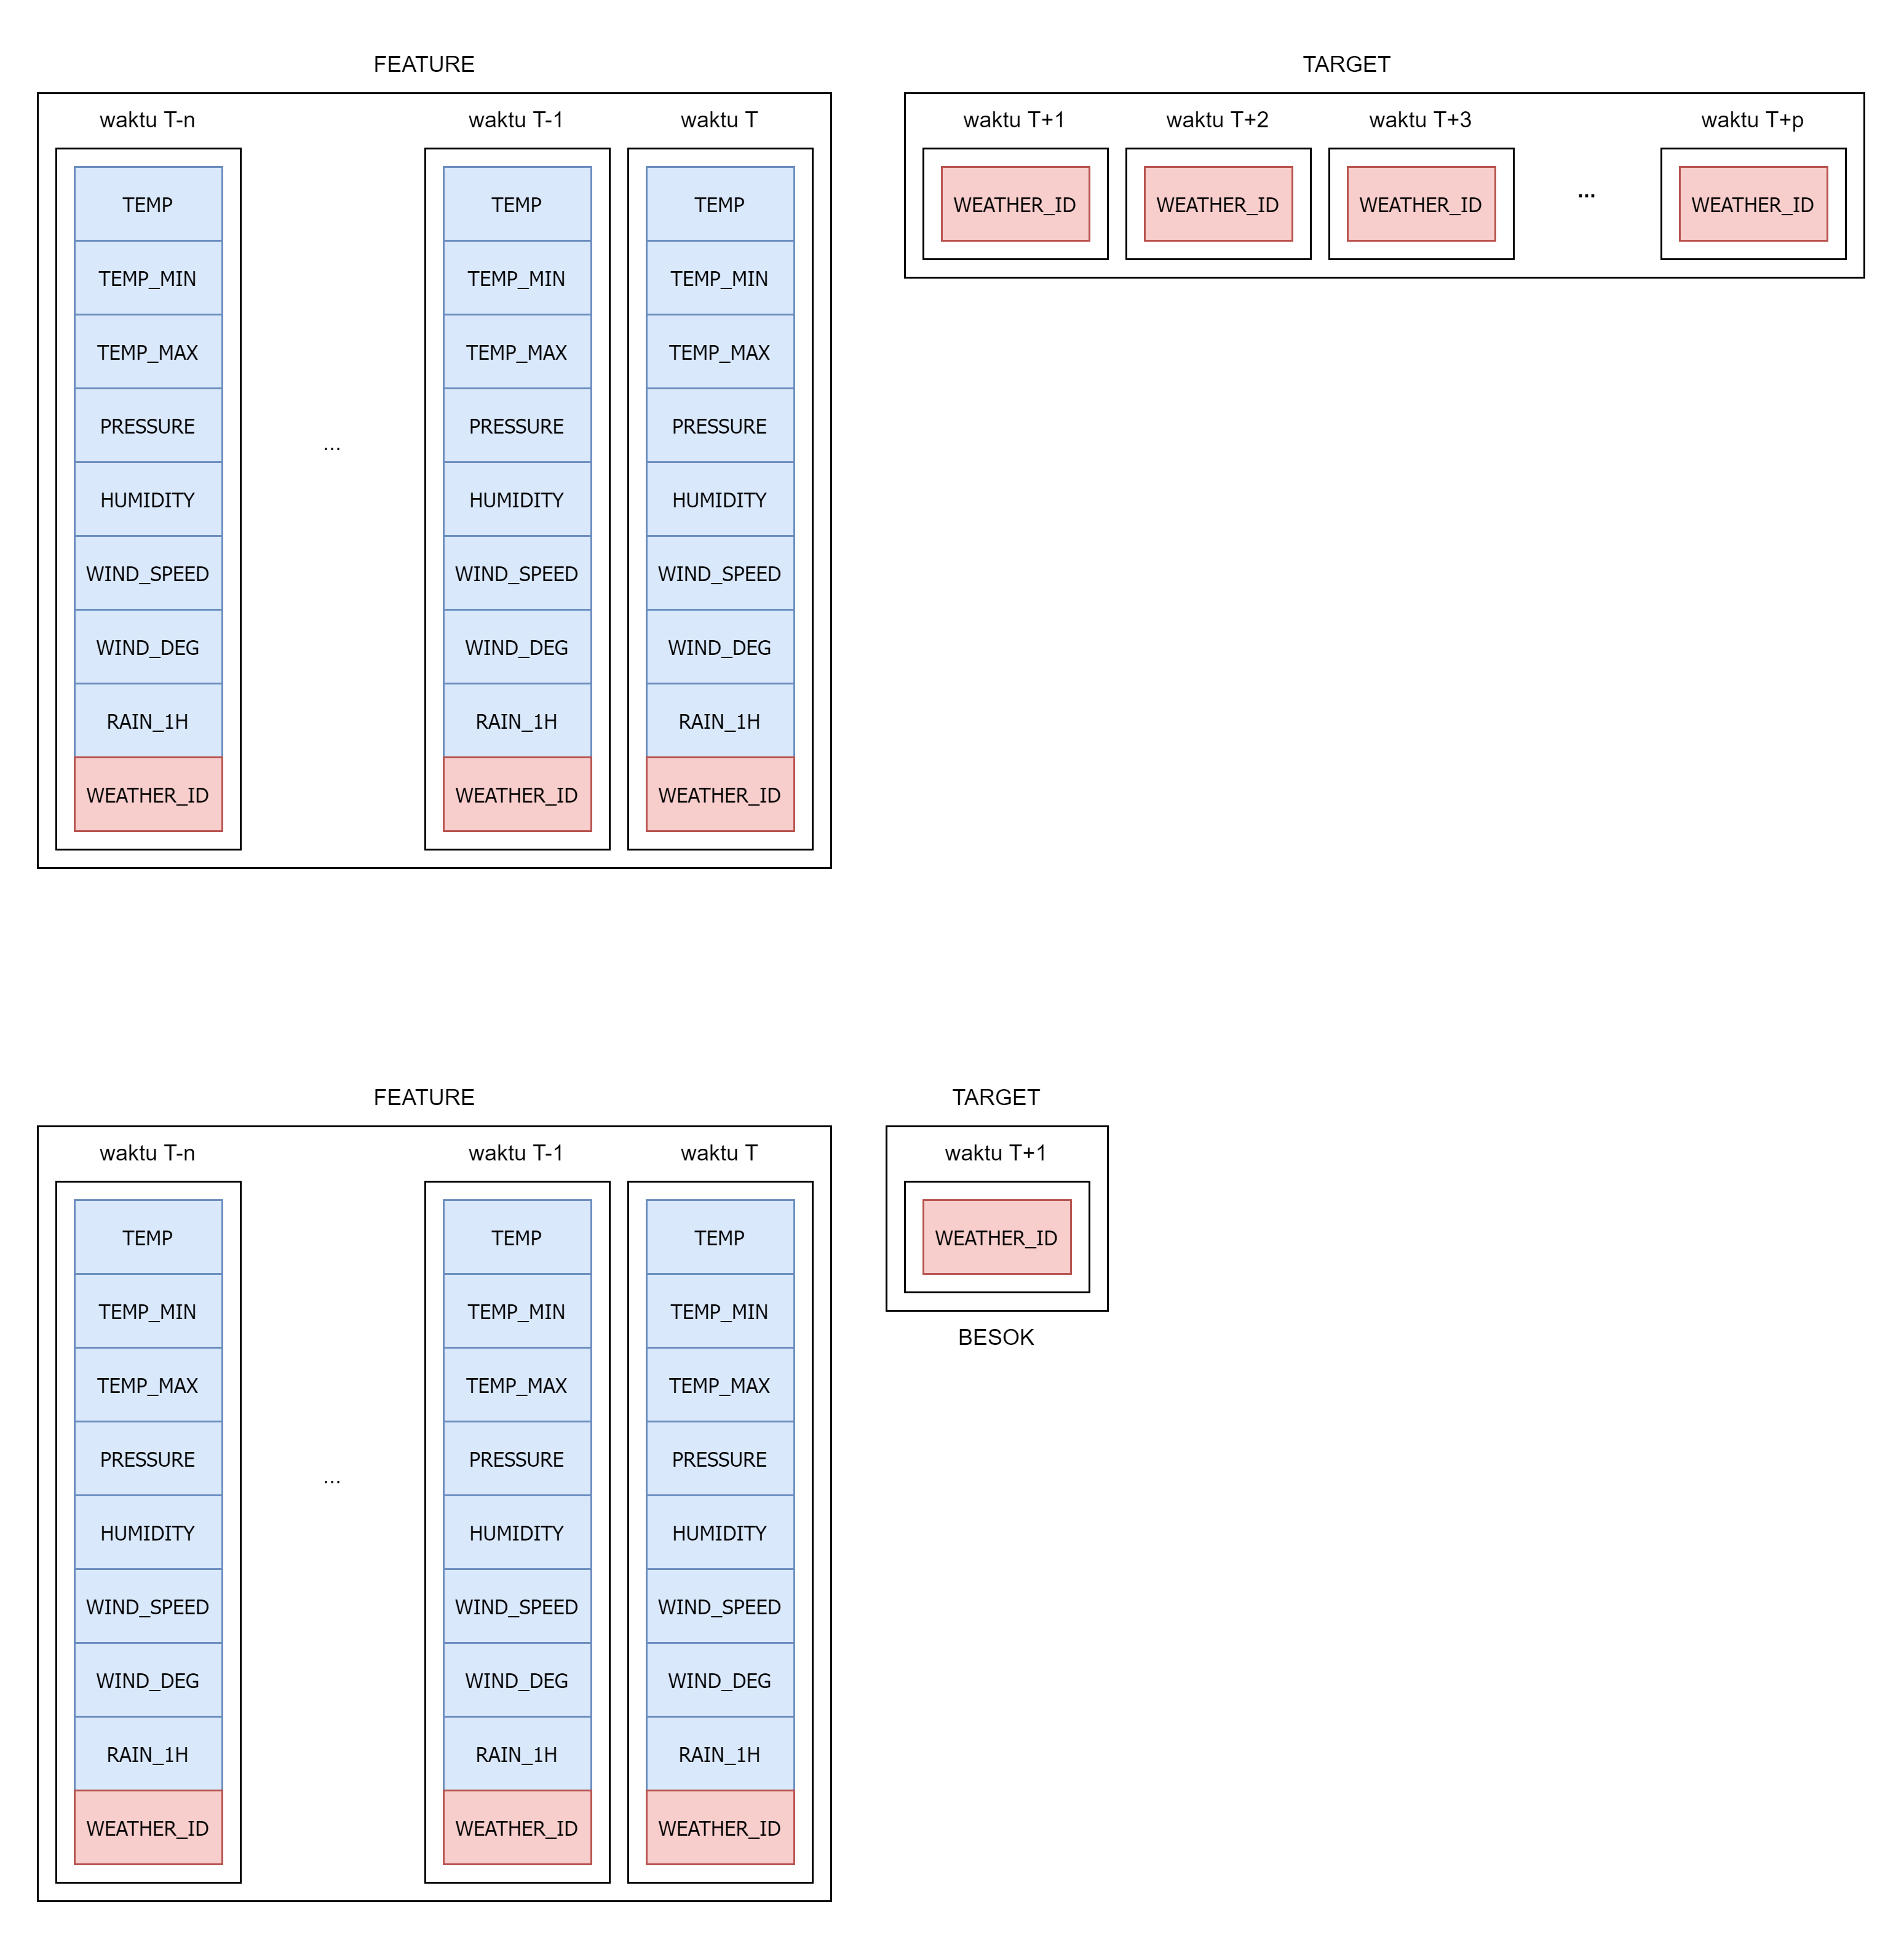
\includegraphics[width=\linewidth]{pert-12.png}
  \caption{Penentuan Awal Parameter Input dan Target}
\end{figure}

\end{document}